%%%%%%%%%%%%%%%%%%%%%%%%%%%%%%%%%%%%%%%%%%%%%%
% Header
\documentclass[11pt]{report}
\usepackage[english]{babel}
\usepackage[utf8x]{inputenc}
\PassOptionsToPackage{hyphens}{url}\usepackage{hyperref}
\usepackage{graphicx}
\usepackage{fullpage}
\usepackage{nicefrac}
\usepackage[lastexercise]{exercise}
\usepackage[dvipsnames]{xcolor}
\usepackage{listings}
\usepackage{enumitem}
\graphicspath{ {./img/} }

\setlength{\parindent}{0cm}

\renewcommand{\ExerciseHeader}{\large\textbf{\ExerciseName~\ExerciseHeaderNB} - \textbf{\ExerciseTitle}\medskip}

\renewcommand{\ExePartHeader}{\medskip\textbf{\ExePartName\ExePartHeaderNB\ExePartHeaderTitle\medskip}}

\begin{document}
%%%%%%%%%%%%%%%%%%%%%%%%%%%%%%%%%%%%%%%%%%%%%%
\title{Exercises -- Week 2: Control Flow}
\subsubsection*{EMAT10007 -- Introduction to Computer Programming}
\subsection*{\Large Exercises -- Week 2. Control Flow}

\subsection*{\Large 2.1 Conditionals}

\subsection*{Essential Questions}

\begin{Exercise}[title=if elif else]  \label{Ex:Numbers}

    \Question{Create two variables, {\tt A} and {\tt B}, and assign a numerical value of your choice to each of the variables. Write a program that tests if {\tt A} - {\tt B}} is positive, negative or zero and prints the outcome of the test to the Console in Spyder. 
    \Question{Create three variables. Each variable should be the name of a student and the value of the variable should be their score in an imaginary assignment e.g {\tt Valentina = 75}. The pass mark for the assignment is 40. Write a program that prints a message telling the user if all, some or none of the students passed the assignment.}
    \Question{Create a variable with a string value. Write a program that prints {\tt`<?> starts with vowel'} if the string begins with a vowel, where {\tt`<?>} is the string value. }
    \Question{A currency trader uses the following equation to calculate the amount in US dollars (USD) for the amount the customer pays in pounds sterling (GBP):
    $$USD = GBP \times M \times R$$
    where $R=1.38$ is the market rate and the multiplier, $M$ is found using the table below, based on the amount paid.:
    
    \begin{center}
    \begin{tabular}{ |l|c| } 
     \hline
     GBP & Multiplier  \\ 
     \hline
     $<$ 50                   & 0.9  \\ 
     $<$ 500 and \geq 50      & 0.92  \\ 
     $<$ 5,000 and \geq 500   & 0.95  \\ 
     $<$ 50,000 and \geq 5000 & 0.97  \\ 
     \geq 50,000              & 0.98  \\ 
     \hline
    \end{tabular}
    \end{center}
    
    Write a program that prints the amount in US dollars for a given amount in pounds sterling, and the effective exchange rate = $\frac{\mbox {USD}}{\mbox {GBP}}$}

\end{Exercise}


\subsection*{Advanced Questions}

\begin{figure}[!h]
        \centering
        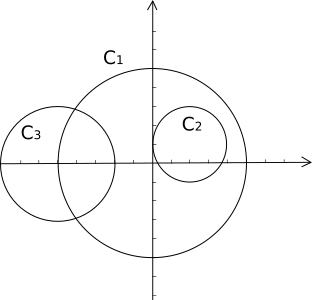
\includegraphics[height=5cm]{circles}
        \caption{Overlapping circles $C_1$, $C_2$ and $C_3$.}
        \label{fig:circles}
\end{figure}

\begin{enumerate}[label=(\Alph*)]
    
    \item Suppose we have three circles in the $xy$-plane (Figure \ref{fig:circles}). 
    
    Circle $C_1$ is centred at $(0, 0)$ with radius of length 5. 
    
    Circle $C_2$ is centred at $(2, 1)$ and has radius of length 2. 
    
    Circle $C_3$ is centred at $(-5, 0)$ and has a radius of length 3. 
    
    Using conditional statements write a program which takes in the variables {\tt x} and {\tt y} and tells the user which circle(s) the point $(x, y)$ is in. 
    
    {\bf Hint:} You can find the Euclidean distance $d$ between two points $(x_1, y_1)$ and $(x_2, y_2)$ by:
    
    $$d = \sqrt{(x_1 - x_2)^2 + (y_1 - y_2)^2}$$ 
    
    How can you make your code as concise as possible? 
    
    Are there any conditions you do not have to test?
\end{enumerate}


    

    % \Question{We can make this code interactive by using the {\tt input()} function. Use the {\tt input()} function to ask the user the age of their cat.}
    % \Question{(*) Can you make a game where a user tries to predict the roll of a dice? Let them know if their guess was too low or too high, and how close it was.
    
    % \textbf{Hint:} Recall you replicated dice throws in Week 1 - Ex.\ref{Ex:Import_Modules}.}



\subsection*{\Large 2.2 User input and nested conditionals}

\subsection*{Essential Questions}

\begin{Exercise}[title= User Input]

    \Question{Write program that asks the user for a number, tests if the number is   positive, negative or zero and prints the outcome of the test to the Console in Spyder.}
    \Question{Write program that asks the user for their name and prints a message telling the user what letter their name ends with e.g. {\tt Your name ends with the letter a}

\end{Exercise}


\begin{Exercise}[title= Nested conditionals]
\label{Ex:Nested_conditionals}

    \Question{Create a variable that asks the user for the name of an imaginary student, then asks the user for the student's score in an imaginary assignment. The pass mark for the assignment is 40. Write a program that prints a message telling the user if the student has passed or failed, and if they have passed, also prints their grade.
    
    \begin{center}
    \begin{tabular}{ |l|c| } 
     \hline
     Score & Grade  \\ 
     \hline
     \geq 70                  & A  \\ 
     $<$ 70 and \geq 60       & B  \\ 
     $<$ 60 and \geq 50       & C  \\ 
     $<$ 50 and \geq 40       & D  \\ 
     $<$ 40                   & Fail  \\ 

     \hline
    \end{tabular}
    \end{center}
    
    }
    
    \Question{Build a text based adventure game by writing a program to execute the flow diagram shown in Figure \ref{fig:adventure}. Your program should ask the user questions and you should use conditionals and nested conditionals to determine the flow of the game.}\label{Q:adventure}

\end{Exercise}

\begin{figure}[h]
        \centering
        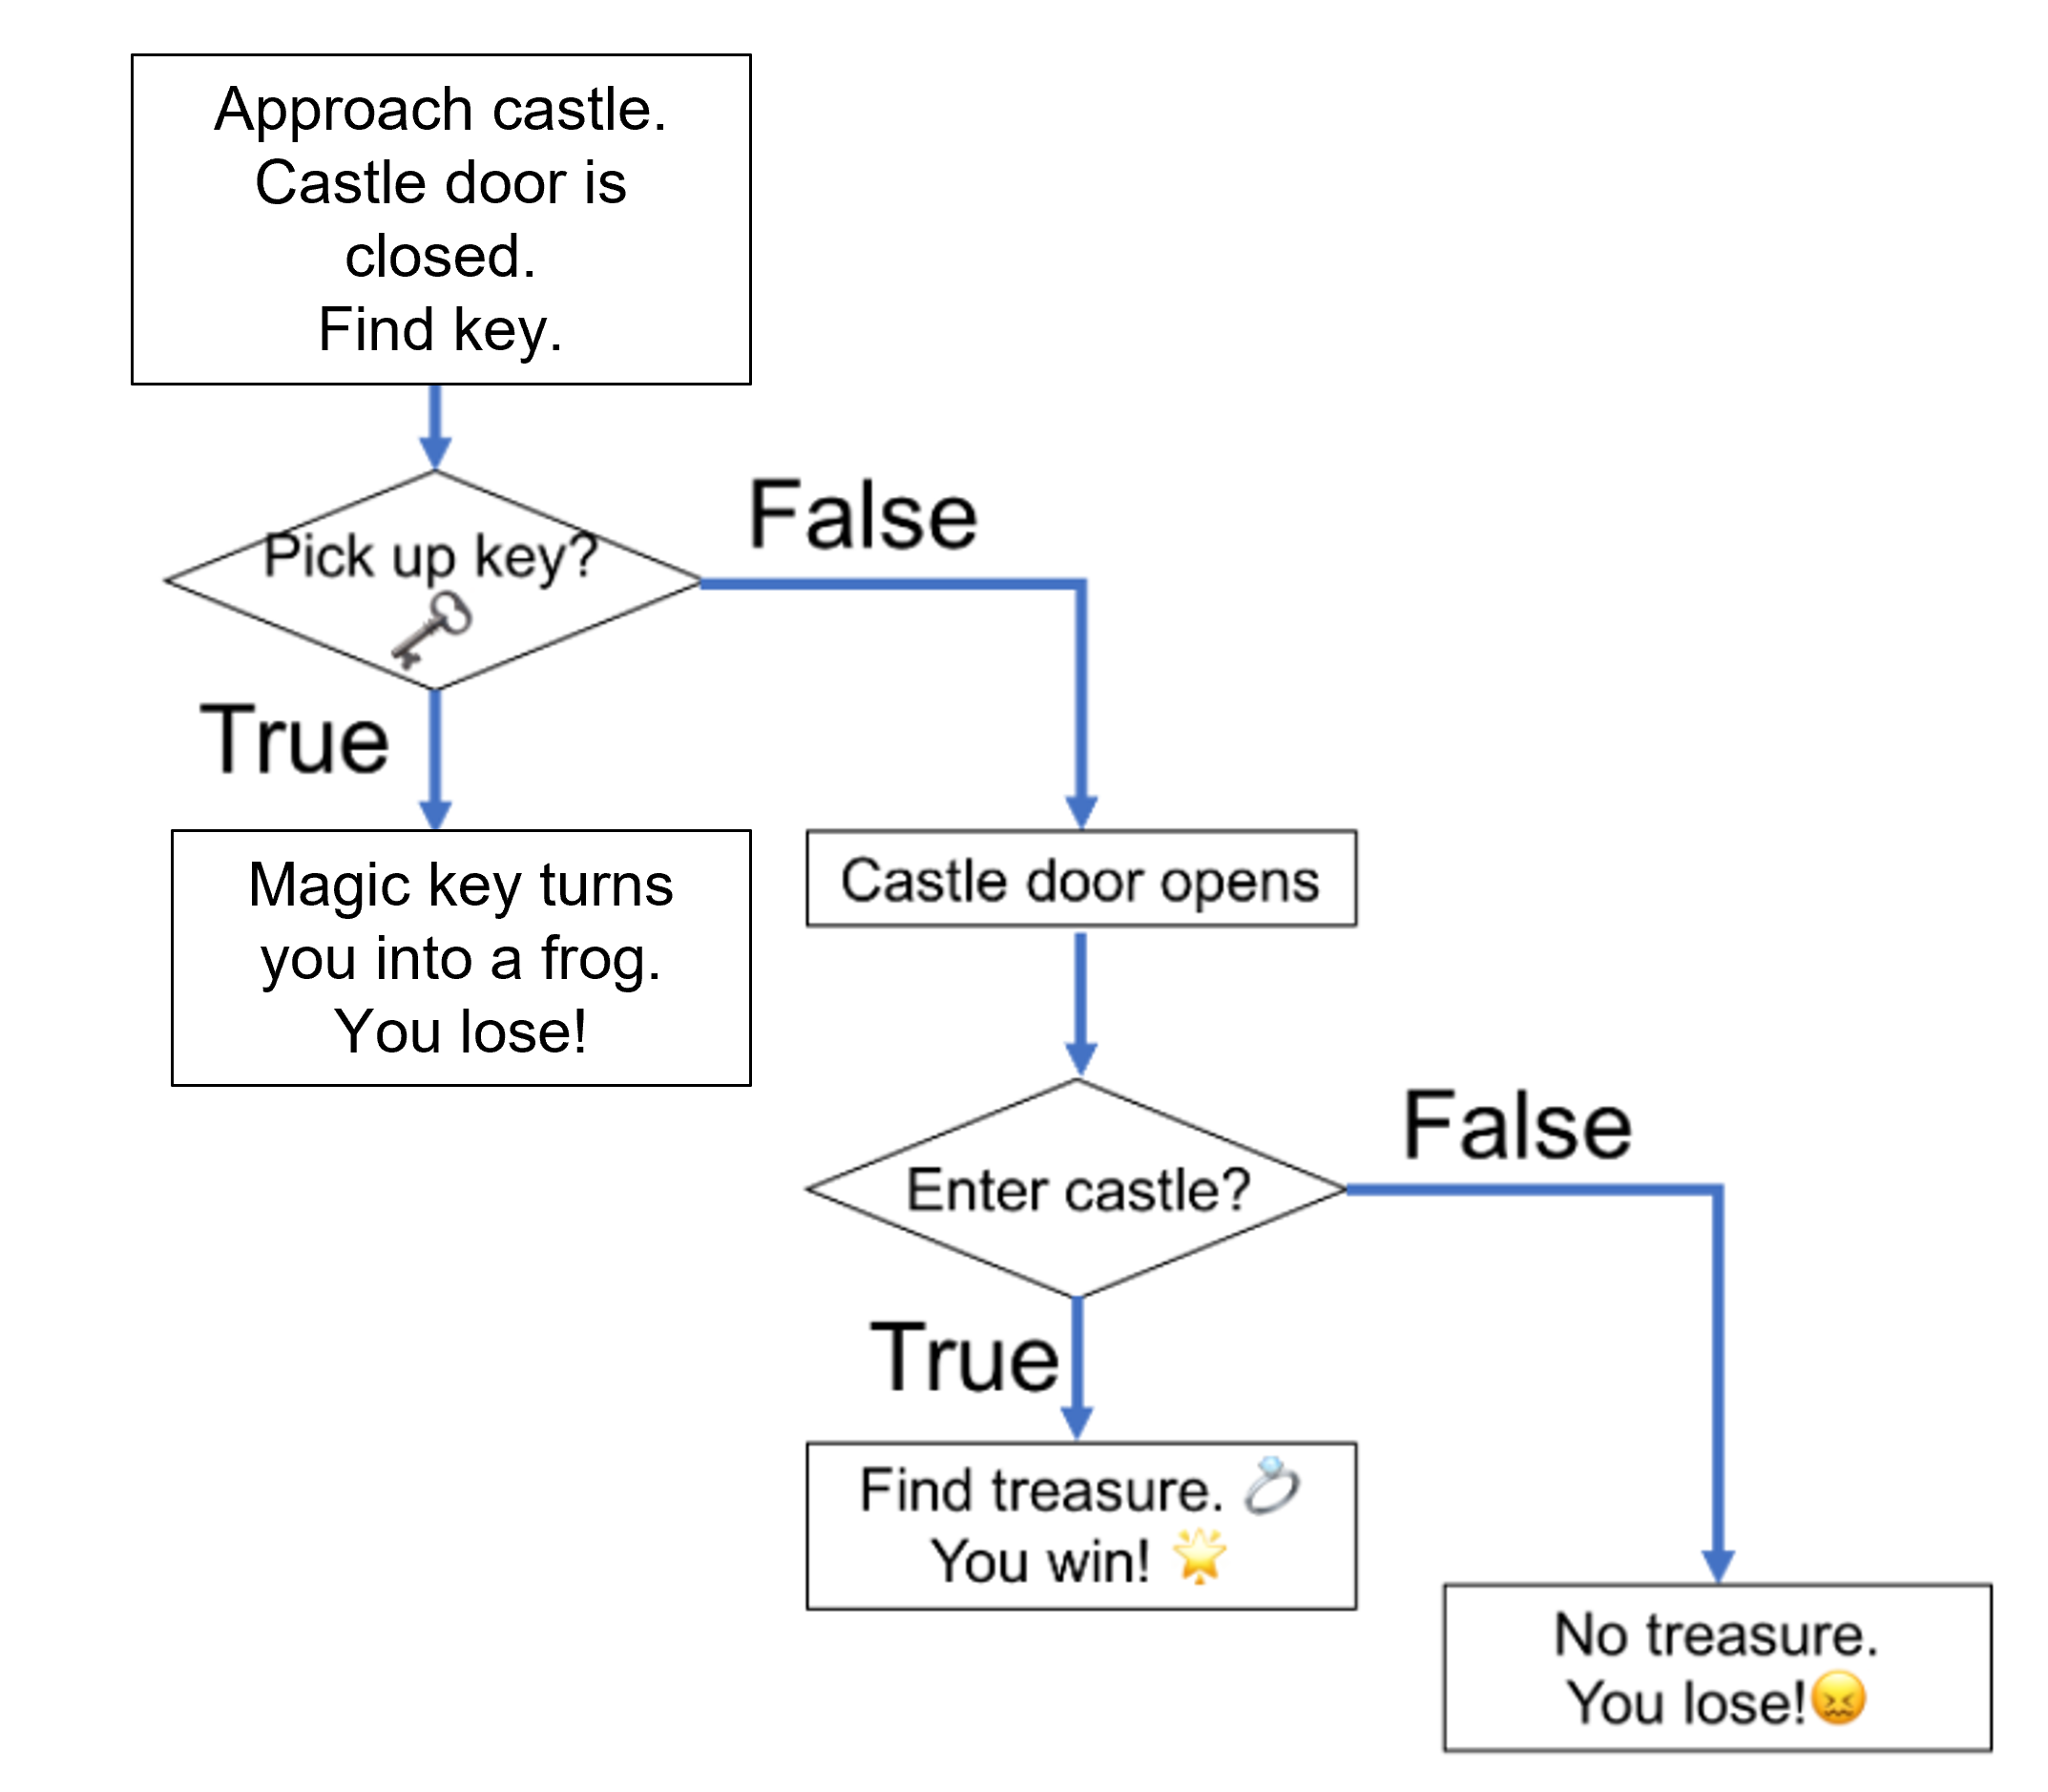
\includegraphics[height=8cm]{adventure}
        \caption{Flow diagram showing an example game}
        \label{fig:adventure}
\end{figure}


\subsection*{Advanced Questions}

\begin{enumerate}[label=(\Alph*)]

    \item Create two variables, {\tt Day} and {\tt Time}. Write a program that tells you which class you should be in based on the day of the week and time of day. Come up with a suitable output for periods where there are no classes. 
    
    \item Build your own text based adventure game in the style of the answer to Exercise \ref{Ex:Nested_conditionals}.\ref{Q:adventure}. Your program should ask the user questions and you should use conditionals and nested conditionals to determine the flow of the game. 
    
\end{enumerate}



\subsection*{Checklist}
\begin{itemize}
	\item Check that you understand the basics: conditional statements (if, elif, else) as well as user input and nested condtiionals.
	\item Finish any incomplete Essential exercises for homework. 
	\item Attend the drop-in session for one-to-one support from a Teaching Assistant if there was anything you didn't understand.
\end{itemize}

\end{document}